
% This is a simple template for a LaTeX document using the "article" class.
% See "book", "report", "letter" for other types of document.

\documentclass[10pt]{article} % use larger type; default would be 10pt

\usepackage[T1]{fontenc}
\usepackage[french]{babel}
\usepackage[utf8]{inputenc} % set input encoding (not needed with XeLaTeX)
\usepackage{kpfonts}
\usepackage{hyperref}
\usepackage{listings}

%%% Examples of Article customizations
% These packages are optional, depending whether you want the features they provide.
% See the LaTeX Companion or other references for full information.

%%% PAGE DIMENSIONS
\usepackage{geometry} % to change the page dimensions
\geometry{a4paper} % or letterpaper (US) or a5paper or....
% THE MARGINS FOR DSA is 1.5cm
\geometry{margin=1.5cm} % for example, change the margins to 2 inches all round
% \geometry{landscape} % set up the page for landscape
%   read geometry.pdf for detailed page layout information


% \usepackage[parfill]{parskip} % Activate to begin paragraphs with an empty line rather than an indent

%%% PACKAGES
\usepackage{booktabs} % for much better looking tables
\usepackage{array} % for better arrays (eg matrices) in maths
\usepackage{paralist} % very flexible & customisable lists (eg. enumerate/itemize, etc.)
\usepackage{verbatim} % adds environment for commenting out blocks of text & for better verbatim
% \usepackage{subfig} % make it possible to include more than one captioned figure/table in a single float
% These packages are all incorporated in the memoir class to one degree or another...

%%% HEADERS & FOOTERS
\usepackage{fancyhdr} % This should be set AFTER setting up the page geometry
% \pagestyle{fancy} % options: empty , plain , fancy

\usepackage{graphicx} % support the \includegraphics command and options
\usepackage{subcaption}
\usepackage{caption}

\usepackage{dingbat} % For the pointy hands
\usepackage{pifont}
% \usepackage{xcolor} % For pretty colors
\usepackage[table]{xcolor}
\usepackage{tikz} % for nice pictures
\usepackage{blindtext}
\usepackage{wrapfig}
\usepackage{gensymb}
% \usepackage{table}

% COLORs
\definecolor{mygold}{RGB}{182, 153, 45}
\definecolor{mygreen}{RGB}{62, 171, 0}
\definecolor{dullgreen}{RGB}{165, 181, 45}
\definecolor{mypurp}{RGB}{84, 45, 181}


% \renewcommand{\headrule}{\color{gray}}
\renewcommand{\headrule}{\hbox to\headwidth{%
  \color{gray}\leaders\hrule height \headrulewidth\hfill}}

\renewcommand{\footrulewidth}{1pt}
% \renewcommand{\footrule}{\hbox to\headwirth{
%     \color{gray}\leaders\hrule height \footrulewidth\hfill}}

\renewcommand{\footrule}{{\color{gray}\vskip-\footruleskip\vskip-\footrulewidth \hrule width\headwidth height\footrulewidth\vskip\footruleskip}}

\fancyhf{}
\rhead{\textcolor{gray}{Séance TP 1}}
\chead{\color{gray} Travaux Pratiques}
% \lhead{Optimisation du GCC}
\lfoot{\color{gray}\textcopyright 2022 Evan Voyles}
\rfoot{\color{gray} Page \thepage\ sur 3}
\cfoot{\color{gray}Spécialité MAIN-3}
\footskip = 0pt
% \voffset = 10pt
% \headsep = 0pt
% \cfoot{\thepage\ of \pageref{LastPage}}

% \renewcommand{\headrulewidth}{0pt} % customise the layout...
% \lhead{}\chead{}\rhead{}
% \lfoot{}\cfoot{\thepage}\rfoot{}


\usepackage[absolute,overlay]{textpos} % Add text in any arbitrary position

%%% SECTION TITLE APPEARANCE
\usepackage{sectsty}
\allsectionsfont{\sffamily\mdseries\upshape} % (See the fntguide.pdf for font help)
% (This matches ConTeXt defaults)

%%% ToC (table of contents) APPEARANCE
\usepackage[nottoc,notlof,notlot]{tocbibind} % Put the bibliography in the ToC
\usepackage[titles,subfigure]{tocloft} % Alter the style of the Table of Contents
\renewcommand{\cftsecfont}{\rmfamily\mdseries\upshape}
\renewcommand{\cftsecpagefont}{\rmfamily\mdseries\upshape} % No bold!

%%% END Article customizations

%%% The "real" document content comes below...

\newcommand{\asgold}[1]{\textcolor{mygold}{{\bf#1}}}
\newcommand{\asgrey}[1]{\textcolor{gray}{{\bf#1}}}
\newcommand{\asred}[1]{\textcolor{red}{{\bf#1}}}
\newcommand{\asor}[1]{\textcolor{orange}{{\bf#1}}}
\newcommand{\ascy}[1]{\textcolor{cyan}{{\bf#1}}}
\newcommand{\asgr}[1]{\textcolor{mygreen}{{\bf#1}}}
\newcommand{\aspurp}[1]{\textcolor{mypurp}{{\bf#1}}}


\begin{document}

% \vspace{-10pt}
% This is the PERFECT SCALING, now we need to adjust the scale a little bit.
\begin{tikzpicture}[remember picture,overlay,yshift=-.2cm, xshift=1.75cm] % LMAOOOOOO This is the EXACT POSITION!!!!
    \node at (0,0) {
\includegraphics[width=4.0cm,height=1.6cm]{media/1280px-Logo_Polytech_Sorbonne.png}};
\end{tikzpicture}

% \hspace{-5cm}
% \hspace{-1cm}
% \hspace{-1cm}

\vspace{-1cm}
\vspace{0.3cm}

{\raggedleft \color{mygold} Algorithmique générale\\
MAIN-3, année 2022\\
Séance TP N\degree 4\\
Avril 2022\\
VOYLES Evan\\}

% This vspace accomodates my name
\vspace{-0.42cm}
\vspace{1.23cm}

{\Large \noindent \color{mygold} Objectif}

{\color{mygold}\noindent\rule{\textwidth}{1pt}}
\vspace{0cm}
\begin{itemize}
    \item[{\color{mygold}\ding{43}}] Arbres binaires équilibrés et balisés.
\end{itemize}

\vspace{1.2cm}
{\color{dullgreen}\noindent \Large \bf Problème}

\vspace{-0.28cm}
{\vspace{0cm}\color{dullgreen}\noindent\rule{\textwidth}{1pt}}

\begin{textblock*}{8.75cm}(12.76cm,7.2cm) % {block width} (coords)
    \Large \aspurp{[Arbres équilibrés balisés]}
\end{textblock*}

\vspace{1cm}

La documentation générale pour ce travail se trouve \href{https://polytech-sorbonne-main-tp2.readthedocs.io/en/latest/}{ici}, la documentation
technique se trouve \href{https://ejovo13.github.io/DSA_TP1/}{là}, et \href{https://github.com/ejovo13/DSA_TP1}{voici} le répertoire git.

\vspace{1cm}
\noindent \asgold{Préliminaires :} \aspurp{Structure Arbre AVL}

J'ai choisi d'implémenté un arbre AVL pour avoir une ABR qui s'équilibre après chaque insertion. La définition de cette structure est nommé \texttt{Node} dans le
code écrit pour ce TP.

Afin d'implémenter un arbe qui s'équilibre, on aura besoins de quelques fonctions qui transforment un arbre binaire de recherche. Les deux qu'on va en servir sont des
rotations dites "à gauche" et "à droite". Dans le code on parle des fonctions \texttt{rotLeft} et \texttt{rotRight}. Examinons ce qui se passe après une rotation.

\begin{figure}[h!]
    \centering
    \begin{subfigure}{.5\textwidth}
      \centering
      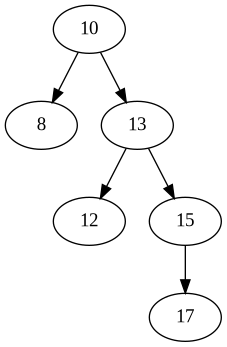
\includegraphics[height=.4\linewidth]{media/tex_1.png}
      \caption{un arbre binaire de recherche non équilibré}
      \label{fig:sub1}
    \end{subfigure}%
    \begin{subfigure}{.5\textwidth}
      \centering
      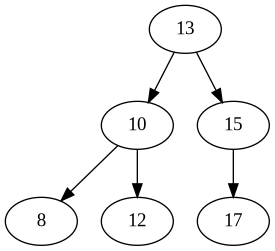
\includegraphics[width=.4\linewidth]{media/tex_1_rot.png}
      \caption{Après rotation à gauche autour du noeud 13}
      \label{fig:sub2}
    \end{subfigure}
    \caption{Un ABR qui se transforment en ARBE. On remarque qu'on a changé les facteurs d'équilibre de les noeuds pour que chaque noeurd vérifié
    l'invariant $\epsilon(T) \in \{-1, 0, 1\}$, ou $\epsilon(T)$ est la facteur de déséquilibre d'un sousarbre.}
    \label{fig:test}
    \end{figure}

Vérifiant cet invariant, on dit que l'arbre dans Figure 1b est \textit{équilibré}. On rajoute la transformation de rotation à gauche ce qui est en
effet l'inverse de l'opération de rotation à droite. Pour aborder l'insertion d'un arbre AVL, on s'en sert de plusiers fonctions d'utilité comme
\texttt{addKeyBST}, une fonction pour insérer un élément dans un ABR ordinaire. On aura des autres fonctions telles que \texttt{updateAVL} qui calcule
la facteur de déséquilibre de chaque noeud, en mettant à jours leurs hauteur. Donc, une insertion à un arbre AVL consiste simplement d'une insertion dans un
ABR et ensuite une étape de réequilibration. Étudions la création d'un arbre AVL à partir des éléments dans l'ensemble : $\{1, 4, 8, 3, 19, 30, 28, 37, 16, 40\}$.

% \begin{figure}[h!]
%     \centering
%     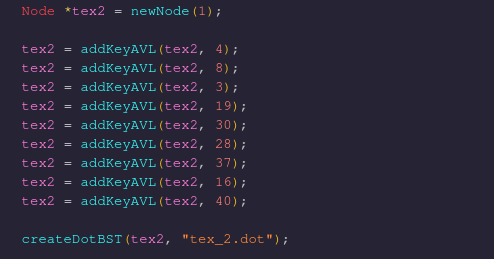
\includegraphics[height=4cm]{media/tex_2_source.png}
%     \caption{Caption}
%     \label{fig:tex_2}
% \end{figure}

\begin{figure}[h!]
    \centering
    \begin{subfigure}{.5\textwidth}
      \centering
      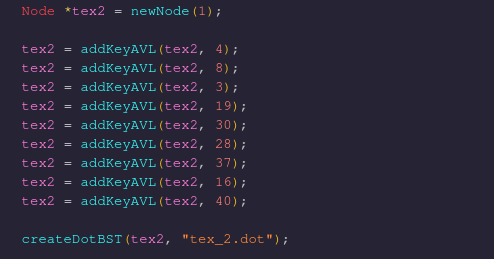
\includegraphics[height=3.5cm]{media/tex_2_source.png}
      \caption{Code pour insérer des éléments dans un arbre AVL}
      \label{fig:tex2_source}
    \end{subfigure}%
    \begin{subfigure}{.5\textwidth}
      \centering
      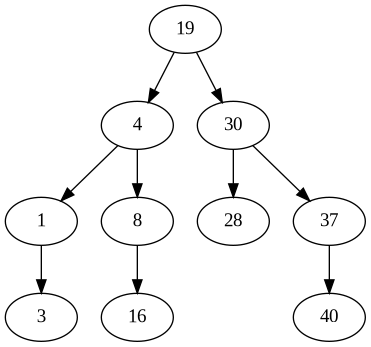
\includegraphics[width=.4\linewidth]{media/tex_2.png}
      \caption{ABRE résultant}
      \label{fig:tex2_dot}
    \end{subfigure}
    % \caption{}
    \label{fig:tex_2}
    \end{figure}



\vspace{1cm}
\noindent \asgold{Partie A :} \aspurp{Structure Arbre Balisé}

\begin{itemize}
    \item[1.] implémenter une procédure \texttt{versAbreBalise} permettant de transformer une ABRE, donnée en argument, en un
    ARBE-balisé. Cette procédure ne retourne aucune valeur! Quelle est la complexité de votre procédure?
\end{itemize}

On note que n'importe quel ABR a $n$ noeuds et $n + 1$ feuilles externes. Pour convertir un ABRE à un ABRE-balisé, il s'agit de stocker tous les clés
dans les feuilles externes, dans l'ordre croissant. Alors pour définir la fonction \texttt{toBalise}, on commence par écrire un mécanisme pour
\begin{itemize}
    \item[\ding{43}] avoir une liste des clés dans l'ordre croissant
    \item[\ding{43}] avoir une liste des noeuds avec des feuilles externes
    \item[\ding{43}] mettre les clés dans l'ordre croissant dans les feuilles externes, aussi dans l'ordre croissant.
\end{itemize}

Toute cette fonctionalité est implémentée dans la fonction \texttt{toBalise}.

\begin{itemize}
    \item[2.] Implémenter la procédure \texttt{inserer} qui permet d'insérer un nouveau noeud dans un ARBRE-balisé.
\end{itemize}

Ce comportement est implémenté par \texttt{insertBalise}. On considère le fait que tous les noeuds sont contenu dans leus feuilles
internes d'un ARBE-balisé, ce qui simplifie énormement le logique du code pour le traiter.

\begin{itemize}
    \item[3.] Implémenter la procédure \texttt{supprimer} qui permet de supprimer un noeud.
\end{itemize}

La fonction \texttt{deleteBalise} implémente cette fonctionalité.


\vspace{1cm}
\noindent \asgold{Partie B :} \aspurp{Structure Arbre Balisé}

% \newpage
\end{document}